%%%%%%%%%%%%%%%%%%%%%%%%%%%%%%%%%%%%%%%%%%%%%%%%%%%%%%%%%%%%%%%%%%%%%%%%%%%%%%%%
% ISE Lab -- Knowledge Representation
% Giovanni Ciatto
% Alma Mater Studiorum - Università di Bologna
% mailto:giovanni.ciatto@unibo.it
%%%%%%%%%%%%%%%%%%%%%%%%%%%%%%%%%%%%%%%%%%%%%%%%%%%%%%%%%%%%%%%%%%%%%%%%%%%%%%%%
%\documentclass[handout]{beamer}\mode<handout>{\usetheme{default}}
%
\documentclass[presentation]{beamer}\mode<presentation>{\usetheme{AMSBolognaFC}}
%\documentclass[handout]{beamer}\mode<handout>{\usetheme{AMSBolognaFC}}
%%%%%%%%%%%%%%%%%%%%%%%%%%%%%%%%%%%%%%%%%%%%%%%%%%%%%%%%%%%%%%%%%%%%%%%%%%%%%%%%
\usepackage{ise-lab-common}
\usepackage{eass23-cl-in-mas}
% version
\newcommand{\versionmajor}{1}
\newcommand{\versionminor}{0}
\newcommand{\versionpatch}{0}
\newcommand{\version}{\versionmajor.\versionminor.\versionpatch}
%%%%%%%%%%%%%%%%%%%%%%%%%%%%%%%%%%%%%%%%%%%%%%%%%%%%%%%%%%%%%%%%%%%%%%%%%%%%%%%%
\title[CL in MAS]{On the role of computational logic in MAS}
%
\subtitle{Practice with \twopkt}
%
\author[\sspeaker{\gcShort}]{\speaker{\gcFull} \\ \gcEmail}
%
\institute[\disiShort, \uniboShort]{\disi{} (\disiShort)\\\unibo}
%
\date[EASS 2023 (v.\ \version)]{
    23rd European Agent Systems Summer School
    \\
    July 17, 2023
    \\
    Prague, Czech Republic
    \\
    (version \version)
}
%
%%%%%%%%%%%%%%%%%%%%%%%%%%%%%%%%%%%%%%%%%%%%%%%%%%%%%%%%%%%%%%%%%%%%%%%%%%%%%%%%
\begin{document}
%%%%%%%%%%%%%%%%%%%%%%%%%%%%%%%%%%%%%%%%%%%%%%%%%%%%%%%%%%%%%%%%%%%%%%%%%%%%%%%%

%/////////
\frame{\titlepage}
%/////////

%%===============================================================================
\section*{Outline}
%%===============================================================================
%
%/////////
\frame[c]{\tableofcontents[hideallsubsections]}
%/////////

%===============================================================================
\section{Why CL for MAS?}
%===============================================================================

%/////////
\begin{frame}[c]{Agent}
%
\begin{block}{Insight}
    Any entity capable of \alert{acting}\footnote{``acting'' = ``affecting the environment, and (possibly) the agents therein contained''}
    to reach some \alert{goals}
    %
    \begin{itemize}
        \item while being situated into some \alert{environment}
        %
        \begin{itemize}
            \item which can be both \alert{perceived} and \alert{affected}
        \end{itemize}

        \item possibly, along with other agents
        %
        \begin{itemize}
            \item with which \alert{interaction} is possible
        \end{itemize}
    \end{itemize}
\end{block}
%
\begin{exampleblock}{Examples of agents}
    \begin{multicols}{2}
        \begin{itemize}
            \item human beings
            \item OS processes
            \item OS threads
            \item logic solvers
            \item robots
            \item BDI agents
        \end{itemize}
    \end{multicols}
\end{exampleblock}
%
\end{frame}
%/////////

%/////////
\begin{frame}[c,allowframebreaks]{Intelligence (of Agents)}
%
\begin{block}{Insight}
    Agents are \alert{intelligent} when they have \alert{cognitive capabilities}, and they know when/how to use them to pursue their goal(s)
\end{block}
%
\begin{exampleblock}{Examples of \textbf{cognitive capabilities}}\small
    \begin{itemize}
        \item \alert{perceiving} stimuli and \alert{recognise} abstractions on top of them
        \item \alert{representing knowledge} (e.g. perceptions, abstractions, goals, actions, etc) and \alert{memorising} it for later re-use
        \item \alert{learning} from the experience (i.e. generalise the gathered knowledge)
        \item \alert{planning} courses of action to pursue goals
        \item \alert{reasoning} about knowledge (to \emph{deduce} implicit knowledge, to \emph{induce} new knowledge, to \emph{abduce} hypotheses)
        \item \alert{interact} with other agents to exchange information (goals, knowledge, plans)
        \item etc.
    \end{itemize}
\end{exampleblock}
%
\begin{exampleblock}{Examples of intelligent agents}
    \begin{itemize}
        \item human agents behave intelligently (most of the times)
        \item software agents require cognitive capabilities, to behave intelligently
        %
        \begin{itemize}
            \item plus some criterion to decide when and how to use them
        \end{itemize}
    \end{itemize}
\end{exampleblock}
%
\framebreak
%
\begin{alertblock}{Cognitive capabilities $\nRightarrow$ Intelligence}
    Cognitive behaviours may or may not be considered as intelligent depending on the \alert{context} they are applied into, and on the \alert{observer}
\end{alertblock}
%
\begin{exampleblock}{Examples of intelligent agents}
    \begin{itemize}
        \item agent stepping through the window at ground floor
        \item agent stepping through the window at $N^{th}$ floor
    \end{itemize}
\end{exampleblock}
%
\end{frame}
%/////////

%/////////
\begin{frame}[c,allowframebreaks]{Fundamental Mechanisms of Intelligent Systems}
%
\begin{enumerate}
    \item Knowledge representation
    %
    \begin{itemize}
        \item How is information represented to favour memorisation and processing
    \end{itemize}
    %
    \item Inference
    %
    \begin{itemize}
        \item How novel/explicit knowledge is attained from prior/implicit knowledge
    \end{itemize}
    %
    \item Perception / actuation
    %
    \begin{itemize}
        \item How information exchange with the environment occurs
    \end{itemize}
    %
    \item Planning
    %
    \begin{itemize}
        \item How courses of actions (directed towards some goal) are computed
    \end{itemize}
    %
    \item Learning
    %
    \begin{itemize}
        \item How experience is transformed into knowledge
    \end{itemize}
    %
    \item Deliberation
    %
    \begin{itemize}
        \item Where all such aspects are tied together
    \end{itemize}
    %
    \item Environment and artefacts
    %
    \begin{itemize}
        \item Where (inter)actions are coordinated
    \end{itemize}
    %
\end{enumerate}
%
\framebreak
%
\begin{block}{Special guest: \textbf{Explanation}}
    How knowledge is \alert{transferred} from an agent to another
    %
    \begin{itemize}
        \item software to human agent $\leftarrow$ symbolic knowledge \alert{extraction}
        \item human to software agent $\leftarrow$ symbolic knowledge \alert{injection}
    \end{itemize}
\end{block}
%
\begin{block}{Special guest: \textbf{Argumentation}}
    Letting agents reach shared agreements by \alert{arguing}
    %
    \begin{itemize}
        \item reason about how arguments attack each other
        \item reason about when to present an argument to the opponent(s)
    \end{itemize}
\end{block}
%
\end{frame}
%/////////

%/////////
\begin{frame}[c,allowframebreaks]{Orthogonal topics}

Topics necessary to understand two or more mechanisms:

\begin{block}{Data science (a.k.a. machine learning, a.k.a. data mining)}
    The use of statistics and algorithms to extract knowledge out of data
    %
    \begin{itemize}
        \item necessary or useful for:
        \vspace{-10pt}
        \begin{multicols}{2}
            \begin{itemize}
                \item perception
                \item learning
                \item inference
                \item processing
            \end{itemize}
        \end{multicols}
    \end{itemize}
\end{block}
%
\begin{itemize}
    \item we assume students already have a background on this topic
    %
    \begin{itemize}
        \item yet, most relevant aspects may be recalled when needed
    \end{itemize}
\end{itemize}

\begin{block}{Computational Logic}
    The use of logic to \emph{perform} or \emph{reason about} computation
    %
    \begin{itemize}
        \item necessary or useful for:
        \vspace{-10pt}
        \begin{multicols}{2}
            \begin{itemize}
                \item knowledge representation
                \item reasoning
                \item planning
                \item learning
                \item perception
                \item deliberation
            \end{itemize}
        \end{multicols}
    \end{itemize}
\end{block}
%
\begin{itemize}
    \item we provide background on this topic, along the course
\end{itemize}

\end{frame}
%/////////

%===============================================================================
\section{Knowledge Representation}
%===============================================================================


%===============================================================================
\subsection{Premises}
%===============================================================================

\begin{frame}{Lecture Goals}
    \begin{itemize}
        \item Understand basic notions concerning \alert{Horn clauses}
        %
        \begin{itemize}
            \item logic terms (constants, functions, variables)
            \item logic clauses (facts, rules, goals)
            % \item unifiers and substitutions
            % \item unification and MGU
        \end{itemize}

        \vfill

        \item Understand how these notions can be exploited for \alert{knowledge representation}
        %
        \begin{itemize}
            \item data structures representation in logic
            \item propositional vs. relational representations
            \item extensional vs. intensional representations
        \end{itemize}

        \vfill

        \item Understand differences in expressiveness among different logics
        %
        \begin{itemize}
            \item[eg] first-order logic vs. Horn clauses
        \end{itemize}
    \end{itemize}
\end{frame}

\begin{frame}{Motivations}
    \begin{itemize}
        \item Why Horn clauses?
        %
        \begin{itemize}
            \item nice expressiveness-tractability trade-off
            \item basis for Prolog, Datalog and Logic Programming
            \item very well established
            %
            \begin{itemize}
                \item involved in tons of literature, theorems, technologies
            \end{itemize}
        \end{itemize}

        \vfill

        \item Why (symbolic) knowledge representation?
        %
        \begin{itemize}
            \item pre-requisite for reifying many cognitive capabilities in software systems
            %
            \begin{itemize}
                \item[eg] reasoning, planning, deliberation, etc.
            \end{itemize}
            \item pre-requisite for logic programing
            \item both human- and machine-interpretable
        \end{itemize}
    \end{itemize}
\end{frame}

\begin{frame}[allowframebreaks]{Historical Overview}
    \begin{enumerate}
        \item In principle, it was first order logic (FOL)
        %
        \begin{itemize}
            \item very expressive, very flexible
            %
            \begin{itemize}
                \item[eg] (recursive) terms + variabiles + quantitiers + predicates + logic connectives
            \end{itemize}

            \item very hard to find a general \alert{resolution} algorithm for deciding the \alert{satisfiability} of any given FOL formula
        \end{itemize}

        \bigskip

        \item In 1965, Robinson proposes the \alert{SL resolution principle}\ccite{Robinson1965}
        %
        \begin{itemize}
            \item[ie] an algorithm for decising the \alert{unsatisfiability} of FOL formul\ae{} in \alert{Skolemized form}
            %
            \begin{itemize}
                \item[ie] all variables are \alert{universally} quantified at the beginning of the formula
                \item[cf] \uurl{https://mathworld.wolfram.com/SkolemizedForm.html} 
            \end{itemize}

            \item SL = Selective Linear
            \item logic \alert{unification} is a basic mechanism for the resolution principle
        \end{itemize}

        \framebreak

        \item In 1974, Kowalski proposes the SL\alert{D} resolution procedure\ccite{KowVan1970}
        %
        \begin{itemize}
            \item SL\alert{D} = Selective Linear [for] \alert{Definite} [clauses]
            %
            \begin{itemize}
                \item definite clauses $\approx$ Horn clauses
                \item[ie] very restricted subset of FOL, discussed in this lecture
                %
                \item[eg] no quantifiers, no negation, no connectors except conjunction and implication, \ldots
            \end{itemize}
        \end{itemize}

        \bigskip

        \item In the 1970s, first Prolog implementations appear
        %
        \begin{itemize}
            \item essentially reifying the SLD procedure into a programming language
            %
            \begin{itemize}
                \item cf. \cite{Korner2022} for the full history
            \end{itemize}
            \item that impacted virtually any subsequent logic/symbolic AI technology
        \end{itemize}

        \framebreak

        \item In 1978, Clark proposes extends SLD with \alert{negation as failure}\ccite{Clark1978} (NaF)
        %
        \begin{itemize}
            \item adding well-founded negation support
        \end{itemize}

        \bigskip

        \item In 1982, Martelli and Montanari propose an efficient algorithm for unification\ccite{MartelliM82}
        %
        \begin{itemize}
            \item paving the way towards many sorts of automated reasoning algorithms / software
        \end{itemize}

        \bigskip

        \item[$\vdots$]

    \end{enumerate}
\end{frame}

%===============================================================================
\subsection{Main notions}
%===============================================================================

\begin{frame}{Overview}
    \begin{itemize}
        \item[$\rightarrow$] Three main ingredients:
        %
        \begin{description}\small
            \item[terms] --- for representing entities
            \item[predicates] --- for representing statements about entities
            \item[clauses] --- for representing properties of entities or relations among them
        \end{description}

        \vfill

        \item Many ways of representing knowledge through them:
        %
        \begin{description}\small
            \item[extensional vs. intensional] $\approx$ explicitly vs. implicitly
            \item[propositional vs. relational] $\approx$ in tabular form vs. as a graph
        \end{description}

        \vfill

        \item One powerful tool:
        %
        \begin{description}\small
            \item[resolution] --- allowing for \alert{intensional} representations, programming, reasoning, \ldots
        \end{description}

        \vfill

        \item Two fundamental mechanisms for manipulating knowledge:
        %
        \begin{description}\small
            \item[substitution application] $\approx$ rewriting a formula by assigning variables
            \item[most general unifier] $\approx$ computing the substitution making 2 formul\ae{} equal
        \end{description}
    \end{itemize}
\end{frame}

\subsubsection{Terms}

\begin{frame}[allowframebreaks]{Terms}
    \begin{block}{Purpose}\centering
        Terms are symbols representing entities from the \alert{domain of the discourse}
    \end{block}
    %
    \begin{block}{Informal definition}
        Terms can be
        %
        \begin{description}
            \item[constants] --- denoting \alert{individual} / simple entities
            \item[structures\footnote{a.k.a. functions}] --- denoting \alert{composed} / groups of entities
            \item[variables] --- denoting \alert{placeholders} for / reference of \emph{unknown} entities
        \end{description}
    \end{block}
    %
    \begin{alertblock}{Formal syntax\hfill\textbf{\footnotesize(notice the syntactic convention!)}}\label{slide:terms}
        \begin{center}
            $\begin{array}{rcl}
                \meta{Term} & := & \meta{Variable} \mid \meta{Structure} \mid \meta{Constant}
                \\
                \meta{Variable} & := & \variable{X}_1 \mid \variable{X}_2 \mid \variable{X}_3 \mid \ldots
                \\
                \meta{Structure} & := & \meta{Functor} \terminal{(} \meta{Arguments} \terminal{)}
                \\
                \meta{Functor} & := & \functor{f}_1 \mid \functor{f}_2 \mid \functor{f}_3 \mid \ldots
                \\
                \meta{Arguments} & := & \meta{Term} \mid \meta{Term} \terminal{,} \meta{Arguments}
                \\
                \meta{Constant} & := & \meta{Functor} \mid \meta{Number}\mid \meta{Boolean}
                \\
                \meta{Number} & := & \mathbb{R} \qquad \meta{Boolean} :=  \functor{true} \mid \functor{false}
            \end{array}$
        \end{center}
        %
        \begin{itemize}
            \item $\mathcal{X} = \{ \variable{X}_1, \variable{X}_2, \variable{X}_3, \ldots \}$ is a set of \alert{variables names}
            \item $\mathcal{F} = \{ \functor{f}_1, \functor{f}_2, \functor{f}_3, \ldots \}$ is a set of \alert{functors}\footnote{a.k.a. function names/symbols} of given \alert{arities}
            \item $\mathbb{R}$ is the set of real numbers
        \end{itemize}
    \end{alertblock}

    \begin{block}{Syntactical convention}
        \begin{itemize}
            \item $\variable{Variables}$ $\rightarrow$ capitalised italics
            \item $\functor{Functor}$ $\rightarrow$ lowercase monospaced
            \item $\meta{Non\text{-}terminal\ symbols}$ $\rightarrow$ sans-serif, wrapped by angular parenteses
            %
            \begin{itemize}
                \item this is just for grammar definitions
            \end{itemize}
            \item $\mathcal{SYMBOLS\ SET}$ $\rightarrow$ uppercase calligraphic italics
            %
            \begin{itemize}
                \item this is just for theoretical definitions
            \end{itemize}
        \end{itemize}
    \end{block}
\end{frame}

\begin{frame}[allowframebreaks]{Example -- Peano Numbers}
    \begin{exampleblock}{Definition: unary representation of natural numbers, via terms}
        \begin{description}
            \item[$\functor{z}$] $\rightarrow$ zero
            \item[$\functor{s}(\variable{X})$] $\rightarrow$ the successor of some (unknown) number $\variable{X}$
            \item[$\functor{s}(\functor{z})$] $\rightarrow$ the successor zero (a.k.a. 1)
            \item[$\functor{s}(\functor{s}(\functor{z}))$] $\rightarrow$ the successor of the successor of zero (a.k.a. 2)
            \item[$\functor{s}(\functor{s}(\functor{s}(\functor{z})))$] $\rightarrow$ the successor of \ldots
        \end{description}
    \end{exampleblock}
    %
    \begin{exampleblock}{Notice that, in this case:}
        \begin{itemize}
            \item $\functor{z}$ is a constant
            \item $\variable{X}$ is a variable
            \item $\functor{s}(\variable{X})$, $\functor{s}(\functor{z})$, etc. are structures
            \item $\mathcal{F} = \{ \functor{s}, \functor{z} \}$ \hfill {\footnotesize(where $\functor{s}$ is a 1-ary functor, while $\functor{z}$ is 0-ary)}
            \item $\mathcal{V} = \{ \variable{X} \}$
        \end{itemize}
    \end{exampleblock}
\end{frame}

\begin{frame}[allowframebreaks]{Example -- Lists}
    \begin{exampleblock}{Definition: (single-)linked lists\hfill\textbf{\footnotesize(LISP nomenclature\cccite{enwiki:cons})}}
        \begin{description}
            \item[$\functor{nil}$] $\rightarrow$ empty list
            \item[$\functor{cons}(\variable{H}, \variable{T})$] $\rightarrow$ the list whose head is $\variable{H}$ and whose tail is $\variable{T}$
            \item[$\functor{cons}(1, \variable{T})$] $\rightarrow$ the list whose first element is $1$ (and whose tail is $\variable{T}$)
            \item[$\functor{cons}(1, \functor{nil})$] $\rightarrow$ the singleton list $[1]$
            \item[$\functor{cons}(1, \functor{cons}(2, \functor{nil}))$] $\rightarrow$ the list $[1,2]$
            \item[$\functor{cons}(1, \functor{cons}(2, \functor{cons}(3, \functor{nil})))$] $\rightarrow$ the list $[1,2,3]$
        \end{description}
    \end{exampleblock}
    %
    \begin{exampleblock}{Notice that, in this case:}
        \begin{itemize}
            \item $\functor{nil}$ is a constant
            \item $\variable{H}$ and $\variable{T}$ are variables
            \item $\functor{cons}(\variable{H}, \variable{T})$, etc. are structures
            \item $\mathcal{F} = \{ \functor{nil}, \functor{cons} \}$ \hfill {\footnotesize(where $\functor{cons}$ is a binary functor, while $\functor{nil}$ is 0-ary)}
            \item $\mathcal{V} = \{ \variable{H}, \variable{T}\}$
        \end{itemize}
    \end{exampleblock}
    %
    \begin{alertblock}{Fun fact: in Prolog\dots}
        \begin{itemize}
            \item the constant `\alert{$\functor{[]}$}' is used in place of `\alert{$\functor{nil}$}'
            \item the binary functor `\alert{$\functor{.}$}' is used in place of `\alert{$\functor{cons}$}'
            \item `\alert{\pl{[$\variable{H}$ | $\variable{T}$]}}' is syntactic sugar for `\alert{\pl{.($\variable{H}$, $\variable{T}$)}}'
            \item `\alert{\pl{[1, 2, 3]}}' is syntactic sugar for `\alert{\pl{.(1, .(2, .(3, [])))}}'
        \end{itemize}
    \end{alertblock}
\end{frame}

% \subsubsubsection{Ancillary definitions}

\begin{frame}[allowframebreaks]{Groundness}
    \begin{block}{Informal definition}\centering
        A term is \alert{ground} iff it has (i.e. contains) no variable
    \end{block}

    \begin{alertblock}{Inductive definition}
        \begin{itemize}
            \item Any variable $X$ is \emph{not} ground
            \item Any constant $\functor{c}$ is ground
            \item Any $n$-ary structure $\functor{f}(t_1, \ldots, t_n)$ is ground iff \emph{all} terms $t_i$ are ground
        \end{itemize}
    \end{alertblock}

    \begin{exampleblock}{Some examples}
        \begin{description}
            \item[$\functor{z}$] and \alert{$\functor{nil}$} $\rightarrow$ ground
            \item[$\functor{s}(\variable{X})$] $\rightarrow$ non-ground
            \item[$\functor{s}(\functor{z})$] $\rightarrow$ ground
            \item[$\functor{s}(\functor{s}(\functor{z}))$] $\rightarrow$ ground
            \item[$\functor{s}(\functor{s}(\functor{s}(\variable{X})))$] $\rightarrow$ non-ground
            \item[$\functor{cons}(\variable{H}, \variable{T})$] $\rightarrow$ non-ground
            \item[$\functor{cons}(1, \variable{T})$] $\rightarrow$ non-ground
            \item[$\functor{cons}(1, \functor{nil})$] $\rightarrow$ ground
            \item[$\functor{cons}(1, \functor{cons}(2, \variable{X}))$] $\rightarrow$ non-ground
            \item[$\functor{cons}(1, \functor{cons}(\variable{X}, \functor{cons}(3, \functor{nil})))$] $\rightarrow$ non-ground
        \end{description}
    \end{exampleblock}
\end{frame}

\begin{frame}[allowframebreaks]{Herbrand Universe}
    \begin{block}{Informal definition}
        The set of all items which can be represented as terms
        %
        \begin{itemize}
            \item attained by applying all $n$-ary functors to all possible terms, recursively
        \end{itemize}
    \end{block}

    \begin{alertblock}{Inductive definition}\label{slide:herbrand}
        Let $\mathcal{F}$ be the set of all $n$-ary functors s.t. $n \geq 0$ (including constants)
        %
        \begin{itemize}
            \item let $\mathcal{H}_0$ be the set of all constants in $\mathcal{F}$
            \item let $\mathcal{H}_1$ be $\mathcal{H}_0 \cup \{ f(t_1, \ldots, t_n) \mid \forall f \in \mathcal{F}, \forall t_1, \ldots, t_n \in \mathcal{H}_0 \}$
            \item $\vdots$
            \item let $\mathcal{H}_{i+1}$ be $\mathcal{H}_i \cup \{ f(t_1, \ldots, t_n) \mid \forall f \in \mathcal{F}, \forall t_1, \ldots, t_n \in \mathcal{H}_i \}$
            \item $\vdots$
            \item then $\mathcal{H}_\infty$ is the Herbrand universe (spawned by $\mathcal{F}$)
        \end{itemize}
    \end{alertblock}

    \framebreak

    \begin{exampleblock}{Example for Peano numbers ($\mathcal{F} = \{ \functor{z}/0, \functor{s}/1 \}$)}
        \begin{itemize}
            \item $\functor{z}$
            \item $\functor{s}(\functor{z})$
            \item $\functor{s}(\functor{s}(\functor{z}))$
            \item $\functor{s}(\functor{s}(\functor{s}(\functor{z})))$
            \item[$\vdots$]
        \end{itemize}
    \end{exampleblock}

    \begin{exampleblock}{Example for lists ($\mathcal{F} = \{ \functor{nil}/0, \functor{cons}/2 \}$)}
        \begin{itemize}
            \item $\functor{nil}$
            \item $\functor{cons}(\functor{nil}, \functor{nil})$
            \item $\functor{cons}(\functor{cons}(\functor{nil}, \functor{nil}), \functor{nil})$
            \item $\functor{cons}(\functor{nil}, \functor{cons}(\functor{nil}, \functor{nil}))$
            \item $\functor{cons}(\functor{cons}(\functor{nil}, \functor{nil}), \functor{cons}(\functor{nil}, \functor{nil}))$
            \item[$\vdots$]
        \end{itemize}
    \end{exampleblock}

    \begin{alertblock}{Important take away}
        As soon as $\mathcal{F}$ contains \emph{at least}
        %
        \begin{itemize}
            \item one constant
            \item and one $n$-ary functor s.t. $n>0$
        \end{itemize}
        %
        the Herbrand base becomes of \alert{infinite} cardinality
    \end{alertblock}

    \begin{block}{Herbrand of \textbf{infinite} cardinality: implications}
        \begin{itemize}
            \item infinitely many terms can be represented
            \item attempts to enumerate them all won't terminate
            \item attempts to store them all will saturate the space
        \end{itemize}
    \end{block}
\end{frame}

\subsubsection{Predicates}

\begin{frame}[allowframebreaks]{Predicates}
    \begin{block}{Purpose}\centering
        Asserting statements about entities from the \alert{domain of the discourse}
    \end{block}
    %
    \begin{block}{Informal definition}
        A \alert{statement} about $n\geq 0$ \alert{terms}, which may or may not hold true
    \end{block}
    %
    \begin{alertblock}{Formal syntax\hfill\textbf{\footnotesize(notice the syntactic convention!)}}\label{slide:predicate}
        $$\begin{array}{rcl}
            \meta{Predicate} & := & \top \mid \bot \mid \meta{Predication} \mid \meta{Predication} \terminal{(} \meta{Arguments} \terminal{)}
            \\
            \meta{Predication} & := & \predication{p}_1 \mid \predication{p}_2 \mid \predication{p}_3 \mid \ldots
            \\
            \meta{Arguments} & := & \meta{Term} \mid \meta{Term} \terminal{,} \meta{Arguments}
            \\
            \meta{Term} & := & \text{see slide \ref{slide:terms}}
        \end{array}$$
        %
        \begin{itemize}
            \item $\mathcal{P} = \{ \predication{p}_1, \predication{p}_2, \predication{p}_3, \ldots \}$ is a set of \alert{predications}\footnote{a.k.a. predicate names/symbols} of given \alert{arities}
            \item \alert{$\top$} denotes the predicate which \alert{always} holds true (a.k.a. \alert{tautology})
            \item \alert{$\bot$} denotes the predicate which \alert{never} holds true (a.k.a. \alert{contradiction})
        \end{itemize}
    \end{alertblock}
    %
    \begin{block}{Syntactical convention}
        \begin{itemize}
            \item $\predication{predication}$ $\rightarrow$ lowercase italics
        \end{itemize}
    \end{block}
\end{frame}

\begin{frame}{Example -- Peano numbers}
    \begin{block}{Assumptions}
        \begin{itemize}
            \item $\mathcal{P} = \{ \predication{nat}, \predication{succ} \}$ \hfill {\footnotesize(where $\predication{nat}$ is a 1-ary predication, while $\predication{succ}$ is binary)}
            \item $\predication{nat}$ states that a term denotes a \alert{natural} number
            \item $\predication{succ}$ states that a term is the \alert{natural} of another one
            %
            \begin{itemize}
                \item provided that they are both natural numbers
            \end{itemize}
        \end{itemize}
    \end{block}
    %
    \begin{exampleblock}{Some possible predicates}
        \begin{description}
            \item[$\predication{nat}(\functor{z})$] $\rightarrow$ zero is a natural number
            \item[$\predication{nat}(\functor{s}(\variable{X}))$] $\rightarrow$ given some term $X$, the term $\functor{s}(\variable{X})$ is a natural number
            \item[$\predication{nat}(\functor{s}(\functor{z}))$] $\rightarrow$ one is a natural number
            \item[$\predication{succ}(\functor{s}(\functor{z}), \functor{z})$] $\rightarrow$ one is the successor of zero
            \item[$\predication{succ}(\functor{s}(\variable{X}), \variable{X})$] $\rightarrow$ given some term $X$, the term $\functor{s}(\variable{X})$ its successor
        \end{description}
    \end{exampleblock}
\end{frame}

\begin{frame}{Example -- Lists}
    \begin{block}{Assumptions}
        \begin{itemize}
            \item $\mathcal{P} = \{ \predication{list}, \predication{head} \}$ \hfill {\footnotesize(where $\predication{list}$ is a 1-ary predication, while $\predication{head}$ is binary)}
            \item $\predication{list}$ states that a term denotes a \alert{list}
            \item $\predication{head}$ states that a term is the \alert{head} of another one
            %
            \begin{itemize}
                \item provided that the latter is a list
            \end{itemize}
        \end{itemize}
    \end{block}
    %
    \begin{exampleblock}{Some possible predicates}
        \begin{description}
            \item[$\predication{list}(\functor{nil})$] $\rightarrow$ the empty list is a list
            \item[$\predication{list}(\functor{cons}(\variable{H}, \functor{nil}))$] $\rightarrow$ given some term $H$, the term $\functor{cons}(\variable{H}, \functor{nil})$ is a list
            \item[$\predication{list}(\functor{cons}(\variable{H}, \variable{T}))$] $\rightarrow$ given some terms $H, T$, the term $\functor{cons}(\variable{H}, \variable{T})$ is a list
            \item[$\predication{head}(\variable{H}, \functor{cons}(\variable{H}, \functor{nil}))$] $\rightarrow$ $H$ is the head of the list $\functor{cons}(\variable{H}, \functor{nil})$
            \item[$\predication{head}(\variable{H}, \functor{cons}(\variable{H}, \variable{T}))$] $\rightarrow$ $H$ is the head of the list $\functor{cons}(\variable{H}, \variable{T})$
        \end{description}
    \end{exampleblock}
\end{frame}

\begin{frame}{Important Remark}
    \begin{alertblock}{Predicates vs. structures}
        \begin{itemize}
            \item predicate and structures have a \emph{very} similar \alert{syntax}
            \item however, they are deeply different, \alert{semantically}
            %
            \begin{description}
                \item[terms] represent entities from the domain of the discourse
                %
                \begin{itemize}
                    \item they just exist
                \end{itemize}

                \item[predicates] represent statements about those entities
                %
                \begin{itemize}
                    \item they can either be true or false
                \end{itemize}
            \end{description}
        \end{itemize}
    \end{alertblock}
\end{frame}

\begin{frame}{Predicates and their arities}

    \begin{description}
        \item[0-ary predicate] (a.k.a. \alert{proposition}): denotes a statement which may either hold or not
        %
        \begin{itemize}
            \item e.g. ``it's raining''
        \end{itemize}

        \vfill

        \item[1-ary predicate] (a.k.a. \alert{set} or \alert{type}): denotes a group of items characterised by a given property
        %
        \begin{itemize}
            \item e.g. ``the set of even numbers''
            %
            \begin{itemize}
                \item[ie] ``the set of all numbers $X$ such that $X$ is a multiple of 2''
            \end{itemize}
        \end{itemize}

        \vfill

        \item[$n$-ary predicate] (a.k.a. \alert{relation}): denotes a relationship holding among $n$ entities
        %
        \begin{itemize}
            \item i.e. a group of $n$-uples characterised by a given property

            \item e.g. ``parenthood'' (binary relation)
            %
            \begin{itemize}
                \item[ie] ``the set of all pairs $(X, Y)$ such that $Y$ is a child of $X$''
            \end{itemize}

            \item e.g. ``students' yearly school reports'' (ternary relation)
            %
            \begin{itemize}
                \item[ie] ``the set of all triplets $(X, Y, Z)$ such that $X$ is a student, $Y$ is a course, and $Z$ is the mark of $X$ in $Y$''
            \end{itemize}
        \end{itemize}
    \end{description}
\end{frame}

\subsubsection{Horn Clauses}

\begin{frame}[allowframebreaks]{Horn Clauses}
    \begin{block}{Purpose}\centering
        Defining (a.k.a. expressing, writing) \alert{propositions}, \alert{sets}, or \alert{relations} concerning the entities of the \alert{domain of the discourse}
    \end{block}
    %
    \begin{block}{Informal definition}
        Horn clauses are logic formul\ae{} of three sorts:
        %
        \begin{description}
            \item[facts] --- denoting predicates which are known to hold
            \item[rules\footnote{a.k.a. definite clauses}] --- denoting that a predicate holds true if a number of other predicates hold true
            \item[goals\footnote{a.k.a. directives}] --- denoting a number of predicates to be proven (either true or false)
        \end{description}
    \end{block}
    %
    \begin{block}{Formal definition (pt. 1)}
        Horn clauses are logic statements of the form
        %
        \begin{center}
            $\overbrace{\underbrace{\phi}_{\text{positive literal}} \vee \underbrace{\neg\psi_1 \vee \ldots \vee \neg \psi_n}_{\text{negative literals}}}^{\text{disjunction form}}$
            \qquad $\equiv$\footnote{$(\neg a \vee b) \equiv (a \Rightarrow b)$, cf. \uuurl{http://discrete.openmathbooks.org/dmoi3/sec_propositional.html}} \qquad
            $\overbrace{\underbrace{\phi}_{\text{head}} \Leftarrow \underbrace{\psi_1 \wedge \ldots \wedge \psi_n}_{\text{body}}}^\text{implication form}$
        \end{center}
        %
        \begin{itemize}
            \item[ie] a \alert{disjunction} of \alert{literals} where \emph{at most} one literal is non-negated
            %
            \begin{itemize}
                \item[aka] an \alert{implication} having \emph{at most} 1 post-condition (the \alert{head}) and $n$ pre-conditions in conjunction (the \alert{the body})
            \end{itemize}
            \item where literals $\phi, \psi_1, \ldots, \psi_n$ are \alert{predicates} of any arity
            %
            \begin{itemize}
                \item possibly involving terms of any sorts
            \end{itemize}
        \end{itemize}
    \end{block}
    %
    \begin{block}{Formal definition (pt. 2)}
        Given a Horn clause $\phi \Leftarrow \psi_1 \wedge \ldots \wedge \psi_n$, it is
        %
        \begin{itemize}
            \item a \alert{goal} iff $\phi \equiv \bot$
            %
            \begin{itemize}
                \item[ie] when the head is a contradiction (a.k.a no head)
                \item then the clause is written as `$\Leftarrow \psi_1 \wedge \ldots \wedge \psi_n$'
            \end{itemize}

            \item a \alert{fact} if $n = 1$ and $\psi_1 = \top$
            %
            \begin{itemize}
                \item[ie] when the head is a tautology (a.k.a no body)
                \item then the clause is written as `$\phi$'
            \end{itemize}

            \item a \alert{rule} otherwise
        \end{itemize}
    \end{block}
\end{frame}

\begin{frame}[allowframebreaks]{Logic Theories (a.k.a. Knowledge Bases)}
    \begin{block}{Definition}
        A \alert{set} of formul\ae{} which are known to be true \& \alert{consistent} with each others
        %
        \begin{description}
            \item[set] $\rightarrow$ the order of formul\ae{} doesn't matter
            \item[consistent] $\rightarrow$ (informal) no formula contradicts the others
            %
            \begin{itemize}
                \item[ie] it is not possible to infer $\bot$ from the set of formul\ae{}
                %
                \begin{itemize}
                    \item[!] deciding whether this is the case or not requires some \alert{inference} algorithm
                \end{itemize}
            \end{itemize}
        \end{description}
    \end{block}
    %
    \begin{block}{Syntax for theories of definite clauses}
        \begin{center}
            $\begin{array}{rcl}
                \meta{Theory} & := & \meta{Definite~Clause} \mid \meta{Theory} \meta{Theory}
                \\
                \meta{Definite~Clause} & := & \meta{Rule} \mid \meta{Fact}
                \\
                \meta{Rule} & := & \meta{Head} \terminal{\Leftarrow} \meta{Body} \terminal{\fullstop}
                \\
                \meta{Fact} & := & \meta{Head} \terminal{\fullstop}
                \\
                \meta{Head} & := & \meta{Predicate}
                \\
                \meta{Body} & := & \meta{Predicate} \mid \meta{Body} \terminal{\wedge} \meta{Body}
                \\
                \meta{Predicate} & := & \text{see slide \ref{slide:predicate}}
            \end{array}$
        \end{center}
    \end{block}
\end{frame}

\begin{frame}{Examples -- Peano numbers}
    \begin{exampleblock}{Defining $\predication{nat}/1$ via a theory of definite clauses}
        \begin{description}
            \item[$\predication{nat}(\functor{z})\fullstop$] $\rightarrow$ $\functor{z}$ is a natural number
            \item[$\predication{nat}(\functor{s}(\variable{X})) \Leftarrow \predication{nat}(\variable{X})\fullstop$] $\rightarrow$ for all $\variable{X}$, $\functor{s}(\variable{X})$ is a natural number if $\variable{X}$ is a natural number as well
        \end{description}
    \end{exampleblock}
    %
    \begin{exampleblock}{Defining $\predication{succ}/2$ via a theory of definite clauses}
        \begin{description}
            \item[$\predication{succ}(\functor{s}(\variable{X}), \variable{X}) \Leftarrow \predication{nat}(\variable{X}) \fullstop$] $\rightarrow$ for all $\variable{X}$, $\functor{s}(\variable{X})$ is the successor of $\variable{X}$ if $\variable{X}$ is a natural number
        \end{description}
    \end{exampleblock}
\end{frame}

\begin{frame}{Examples -- Lists}
    \begin{exampleblock}{Defining $\predication{list}/1$ via a theory of definite clauses}
        \begin{description}
            \item[$\predication{list}(\functor{nil})\fullstop$] $\rightarrow$ $\functor{nil}$ is a list
            \item[$\predication{list}(\functor{cons}(\variable{H}, \variable{T})) \Leftarrow \predication{list}(\variable{T})\fullstop$] $\rightarrow$ for all $\variable{T}$ and regardless of $\variable{H}$, $\functor{cons}(\variable{H}, \variable{T})$ is a list if $\variable{T}$ is a list as well
        \end{description}
    \end{exampleblock}
    %
    \begin{exampleblock}{Defining $\predication{head}/2$ via a theory of definite clauses}
        \begin{description}
            \item[$\predication{head}(\variable{H}, \functor{cons}(\variable{H}, \variable{T})) \fullstop$] $\rightarrow$ for all $\variable{H}$ and regardless of $\variable{T}$, the head of $\functor{cons}(\variable{H}, \variable{T})$ is $\variable{H}$
        \end{description}
    \end{exampleblock}
\end{frame}

\begin{frame}[allowframebreaks]{Horn clauses vs. FOL formul\ae}
    \begin{block}{Horn clauses are \textbf{particular cases} of FOL formul\ae, where}
        \begin{itemize}
            \item all variables in the head are \alert{universally} quantified
            \item all variables occurring in the in the body (but not in the head) are \alert{existentially} quantified
            \item where negation of predicates is forbidden
            \item where all logic connectives are forbidden
            %
            \begin{itemize}
                \item except conjunction and implication
                \item implication can only occur once
                \item conjunction can only occur among the pre-conditions of the implication
            \end{itemize}
        \end{itemize}
    \end{block}

    \begin{exampleblock}{How to read definite clauses}
        \centering
        $\predication{mother}(\variable{X}) \Leftarrow \predication{parent}(\variable{X}, \variable{Y}) \wedge \predication{female}(\variable{X})$

        \medskip

        $\downarrow$ {\footnotesize should be read as}

        \medskip

        $\alert{\forall \variable{X}} : \predication{mother}(\variable{X}) \Leftarrow \alert{\exists \variable{Y}} : \predication{parent}(\variable{X}, \variable{Y}) \wedge \predication{female}(\variable{X})$

        \medskip

        $\downarrow$ {\footnotesize i.e., in natural language}

        \medskip

        ``for all $\variable{X}$, $\variable{X}$ is a mother if there exists some $\variable{Y}$ of which $\variable{X}$ is parent, \\ and if $\variable{X}$ is female''
    \end{exampleblock}
\end{frame}

\begin{frame}{Skip to Exercises} 
    \begin{block}{You may already start some exercises}
        \begin{enumerate}
            \item exercise about terms on slide \ref{slide:first-exercise-on-terms}
            \item exercise about Herbrand universe on slide \ref{slide:second-exercise-on-terms}
            \item exercise about clauses on slide \ref{slide:first-exercise-on-clauses}
            \item exercise about theories on slide \ref{slide:second-exercise-on-clauses}
        \end{enumerate}
    \end{block}

    \begin{alertblock}{Prerequisites}
        \begin{itemize}
            \item consider reading slide \ref{slide:prolog} (relevant Prolog-related aspects)
            \item consider reading slide \ref{slide:tuprolog-overview} (relevant \twopkt{}-related aspects)
        \end{itemize}
        before proceeding with exercises
    \end{alertblock}
\end{frame}

%===============================================================================
\subsection{Flexibility of Logic Representation}
%===============================================================================

\begin{frame}{Overview}
    \begin{itemize}
        \item Three main ingredients:
        %
        \begin{description}\small
            \item[terms] --- for representing entities
            \item[predicates] --- for representing statements about entities
            \item[clauses] --- for representing properties of entities or relations among them
        \end{description}

        \vfill

        \item[$\rightarrow$] Many ways of representing knowledge through them:
        %
        \begin{description}\small
            \item[extensional vs. intensional] $\approx$ explicitly vs. implicitly
            \item[propositional vs. relational] $\approx$ in tabular form vs. as a graph
        \end{description}

        \vfill

        \item One powerful tool:
        %
        \begin{description}\small
            \item[resolution] --- allowing for \alert{intensional} representations, programming, reasoning, \ldots
        \end{description}

        \vfill

        \item Two fundamental mechanisms for manipulating knowledge:
        %
        \begin{description}\small
            \item[substitution application] $\approx$ rewriting a formula by assigning variables
            \item[most general unifier] $\approx$ computing the substitution making 2 formul\ae{} equal
        \end{description}
    \end{itemize}
\end{frame}

\subsubsection{Intensional vs. Extensional}

\begin{frame}[allowframebreaks]{Intensional vs. Extensional Representations}
    \begin{block}{``Intension and extension'' \uuurl{https://www.britannica.com/topic/intension}}\itshape\small
        In logic, correlative words that indicate the reference of a term or concept:
        %
        \begin{description}
            \item[``intension''] indicates the internal content of a term or concept that constitutes its formal definition;
            \item[``extension''] indicates its range of applicability by naming the particular objects that it denotes.
        \end{description}
        %
        For instance:
        %
        \begin{itemize}
            \item the intension of ``ship'' as a substantive is ``vehicle for conveyance on water,''
            \item its extension embraces such things as cargo ships, passenger ships, battleships, and sailing ships.
        \end{itemize}
    \end{block}

    \framebreak

    \begin{block}{In practice}\small
        \begin{description}
            \item[intensional] representations of concepts $\approx$ describing the \alert{invariants} all instances must comply to
            %
            \begin{itemize}
                \item support both \alert{generating} (resp. \alert{testing}) instances from (resp. against) definitions
                \item \alert{concise} as information is \alert{implicit}, but \alert{computation} is required
            \end{itemize}

            \item[extensional] representations of concepts $\approx$ describing \alert{actual} instances and their peculiarities
            %
            \begin{itemize}
                \item this is what we do when we ``fill'' data sets/bases with data
                \item information is \alert{explicitly} represented, hence \alert{space} is required
            \end{itemize}
        \end{description}
    \end{block}

    \begin{block}{In computational logic}
        \begin{description}
            \item[variables] make it possible to \alert{express} \emph{intensional} representations
            \item[inference] makes it possible to \alert{exploit} \emph{intensional} representations
        \end{description}
    \end{block}

    \begin{alertblock}{Benefits of intensional representations}
        \begin{itemize}
            \item compactness of representations
            \item possibility to express/treat concepts with \alert{infinitely many} instances
            %
            \begin{itemize}
                \item[eg] Peano numbers: 2 clauses, infinitely many natural numbers!
            \end{itemize}
        \end{itemize}
    \end{alertblock}
\end{frame}

\begin{frame}[allowframebreaks]{Example -- Abraham's Family Tree}
    \begin{figure}
        \centering
        \caption{Abraham's family tree \uuurl{https://en.wikipedia.org/wiki/Abraham\%27s_family_tree}}
        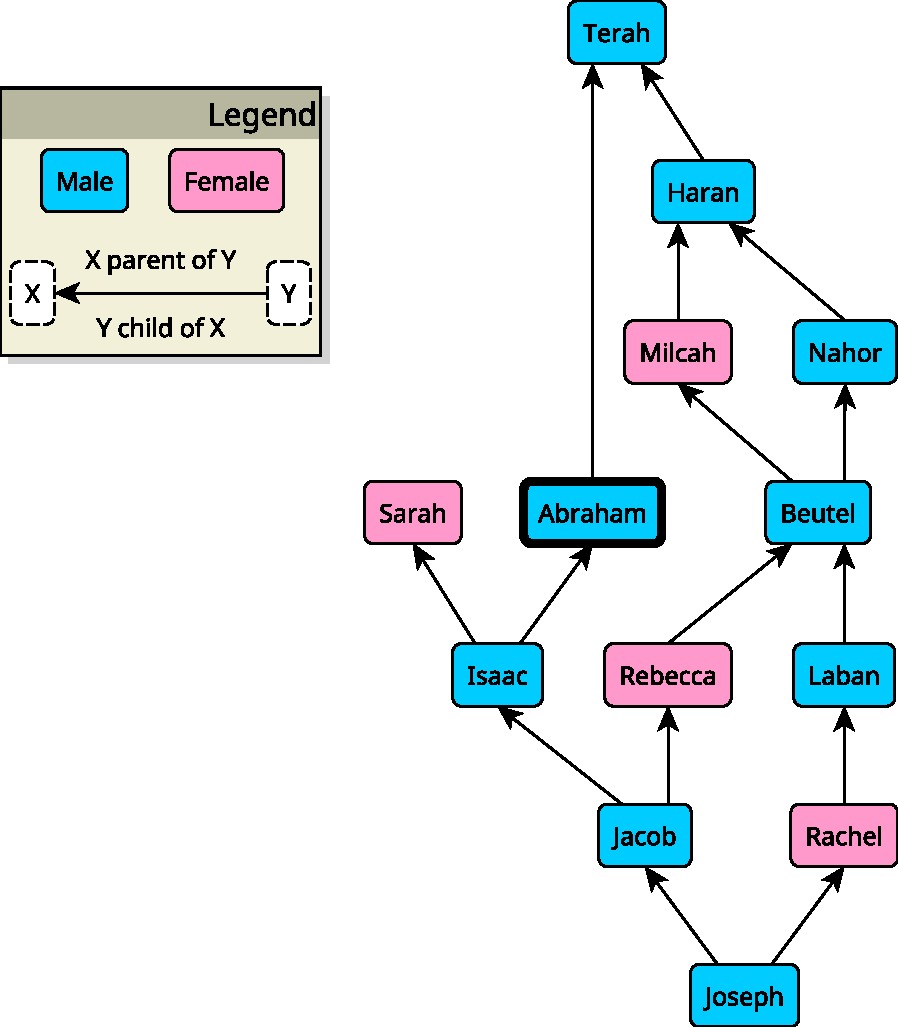
\includegraphics[width=.4\linewidth]{figures/family-tree.pdf}
    \end{figure}

    \framebreak

    \begin{block}{\textbf{Extensional} representation of \textbf{parenthood} (via ground facts)}
        \begin{itemize}
            \item $\predication{parent}(\functor{abraham}, \functor{isaac})\fullstop$
            \item $\predication{parent}(\functor{sarah}, \functor{isaac})\fullstop$
            \item $\predication{parent}(\functor{isaac}, \functor{jacob})\fullstop$
            \item $\predication{parent}(\functor{beutel}, \functor{rebecca})\fullstop$
            \item $\predication{parent}(\functor{rebecca}, \functor{jacob})\fullstop$
            \item[$\vdots$]
        \end{itemize}
    \end{block}

    \framebreak

    \begin{block}{\textbf{Intensional} representation of \textbf{grand-parenthood} (via rules)}
        \begin{itemize}
            \item $\predication{grand\text{-}parent}(\variable{X}, \variable{Y}) \Leftarrow \predication{parent}(\variable{X}, \variable{Z}) \wedge \predication{parent}(\variable{Z}, \variable{Y}) \fullstop$
        \end{itemize}
    \end{block}

    \begin{alertblock}{Important remarks}
        \begin{itemize}
            \item Thanks to \alert{variables}, one may reference unknown entities in clauses
            \item One may need \alert{inference} to actually know who's the grandparent of a given person
            %
            \begin{itemize}
                \item inference $\rightarrow$ computation
            \end{itemize}
            \item Alternatively, one my \alert{extensively} represent grandparenthood instances
        \end{itemize}
    \end{alertblock}
\end{frame}

\subsubsection{Relational vs. Propositional}

\begin{frame}[allowframebreaks]{Relational vs. Propositional Representations}

    \begin{block}{Propositional representations}
        The natural way of representing knowledge in \alert{data science}:
        %
        \begin{itemize}
            \item data is represented in \alert{tabular form}
            %
            \begin{itemize}
                \item \alert{attribute--value}, bi-dimensional representation
                \item $m$ columns, one per attribute
                \item $n$ rows, one per instance
            \end{itemize}

            \item this can be attained $n$ definite clauses, one per instance
            %
            \begin{itemize}
                \item each one having a head of arity $m$
                \item where the $i^{th}$ argument of the head of the $j^{th}$ denotes the value of the $i^{th}$ attribute for the $j^{th}$ instance
            \end{itemize}
        \end{itemize}
    \end{block}

    \begin{exampleblock}{Iris Dataset, in \textbf{propositional} form\cccite{uci:iris}}
        \begin{itemize}
            \item $\predication{iris}(\functor{flower1}, 5.1, 3.5, 1.4, 0.2, \functor{setosa}) \fullstop$
            \item[$\vdots$]
            \item $\predication{iris}(\functor{flower82}, 5.5, 2.4, 3.7, 1.0, \functor{versicolor}) \fullstop$
            \item[$\vdots$]
            \item $\predication{iris}(\functor{flower150}, 5.9, 3.0, 5.1, 1.8,  \functor{virginica}) \fullstop$
        \end{itemize}
    \end{exampleblock}
    %
    \begin{itemize}
        \item Attributes names:
        %
        \begin{itemize}
            \item[1.] identifier, \alert{2.} sepal length, \alert{3.} sepal width, \alert{4.} petal length,
            \item[5.] petal width, \alert{6.} class
        \end{itemize}
    \end{itemize}

    \begin{block}{Relational representations}
        The natural way of representing knowledge in computational logic:
        %
        \begin{itemize}
            \item constants represent individual entities or values
            \item structures represent groups of composed entities
            \item clauses represent sets of, or relations among, those entities
        \end{itemize}
    \end{block}

    \begin{exampleblock}{Iris Dataset, in \textbf{relational} form\cccite{uci:iris}}
        \begin{multicols}{2}
            \begin{itemize}
                \item $\predication{iris}(\functor{flower1}) \fullstop$
                \item $\predication{sepal-length}(\functor{flower1}, 5.1) \fullstop$
                \item $\predication{sepal-width}(\functor{flower1}, 3.5) \fullstop$
                \item $\predication{petal-length}(\functor{flower1}, 1.4) \fullstop$
                \item $\predication{petal-width}(\functor{flower1}, 0.2) \fullstop$
                \item $\predication{class}(\functor{flower1}, \functor{setosa}) \fullstop$
                \item[$\vdots$]
                \item $\predication{iris}(\functor{flower82}) \fullstop$
                \item $\predication{sepal-length}(\functor{flower82}, 5.5) \fullstop$
                \item $\predication{sepal-width}(\functor{flower82}, 2.4) \fullstop$
                \item $\predication{petal-length}(\functor{flower82}, 3.7) \fullstop$
                \item $\predication{petal-width}(\functor{flower82}, 1.0) \fullstop$
                \item $\predication{class}(\functor{flower82}, \functor{versicolor}) \fullstop$
                \item[$\vdots$]
            \end{itemize}
        \end{multicols}
    \end{exampleblock}
\end{frame}

\begin{frame}{Pros and cons}
    \begin{columns}
        \begin{column}{.48\linewidth}
            \begin{block}{Propositional}
                \begin{itemize}
                    \item[$\checkmark$] Table $\rightarrow$ matrix
                    %
                    \begin{itemize}
                        \item[$\rightarrow$] good for sub-symbolic processing
                    \end{itemize}
                    \item[$\checkmark$] Easy to count/add instances
                    \item[$\checkmark$] Easy to count attributes
                    \item[$\times$] Hard to add/remove attributes
                    \item[$\times$] Rigid schema
                \end{itemize}
            \end{block}
        \end{column}
        %
        \begin{column}{.48\linewidth}
            \begin{block}{Relational}
                \begin{itemize}
                    \item[$\checkmark$] Supports $n$-ary relations s.t. $n\geq2$
                    \item[$\checkmark$] Good for symbolic processing
                    \item[$\checkmark$] Easy to count/add instances
                    \item[$\checkmark$] Easy to add/remove attributes
                    \item[$\checkmark$] Flexible schema
                    \item[$\times$] Hard to count attributes
                \end{itemize}
            \end{block}
        \end{column}
    \end{columns}
    %
    \begin{center}
        \alert{easy} $\rightarrow$ O(1)
        \\
        \alert{hard} $\rightarrow$ O(n)
    \end{center}
\end{frame}

\begin{frame}{Relationalisation and Propositionalization\ccite{Lachiche2010}}
    \begin{block}{Relationalisation}
        \begin{itemize}
            \item the operation of converting a propositional theory into a relational one
            \item it is always possible
        \end{itemize}
    \end{block}

    \begin{block}{Propositionalisation}
        \begin{itemize}
            \item the operation of converting a relational theory into a propositional one
            \item may be tricky if the relational theory has $n$-ary relations s.t. $n\geq3$
        \end{itemize}
    \end{block}
\end{frame}

%===============================================================================
\subsection{About Horn Clauses in Prolog}
%===============================================================================

\begin{frame}{Prolog Overview}
\label{slide:prolog}
    \begin{itemize}
        \item Most relevant language in the \alert{logic programming} playground

        \vfill

        \item The \alert{program} is a \alert{theory} of Horn clauses
        %
        \begin{itemize}
            \item exploiting a compact notation (`\pl{:-}' instead of `$\Leftarrow$', `\pl{,}' instead of `$\wedge$')
        \end{itemize}

        \vfill

        \item Execution consists of applying SLD+NaF to prove \alert{goals} against that theory
        %
        \begin{itemize}
            \item goals are user-provided, a.k.a. \alert{queries}
            \item all solutions are \alert{lazily} enumerated via \alert{backtracking}
            \item solutions consists of variables' \alert{assignments}
        \end{itemize}

        \vfill

        \item Several built-in predicates are commonly available for practical reasons
        %
        \begin{itemize}
            \item Prolog is an actual programming language
            \item quite more than a simple theorem prover
        \end{itemize}
    \end{itemize}
\end{frame}

\subsubsection{Why Prolog is tricky}

\begin{frame}[allowframebreaks]{Horn Clauses in Prolog}
    \begin{block}{The Prolog trick}
        \begin{itemize}
            \item the \alert{exact same syntax} is used for both predicates and structures
            \item making them interchangeable
            \item hence supporting the definition of \alert{meta-predicates}
            %
            \begin{itemize}
                \item[ie] predicates accepting other predicates as arguments
            \end{itemize}
        \end{itemize}
    \end{block}

    \prologimport{listings/meta-predicates.pl}

    \begin{block}{Consequences of the Prolog trick}
        \begin{itemize}
            \item conjunctions are represented as structures whose functor is $\pl{,}/2$
            %
            \begin{center}
                \begin{tabular}{rcl}
                    \pl{(a, b)} & \qquad $\equiv$ \qquad & \pl{,(a, b)}
                    \\
                    \pl{(a, b, c)} & \qquad $\equiv$ \qquad & \pl{,(a, ,(b, c))}
                    \\
                    \pl{(a, b, c, d)} & \qquad $\equiv$ \qquad & \pl{,(a, ,(b, ,(c, d)))}
                \end{tabular}
            \end{center}

            \item clauses are represented as structures whose functor is $\pl{:-}/2$
            %
            \begin{center}
                \begin{tabular}{rcll}
                    \pl{a.} & \qquad $\equiv$ \qquad & \pl{:-(a, true)} & fact
                    \\
                    \pl{a :- b.} & \qquad $\equiv$ \qquad & \pl{:-(a, b)} & rule
                    \\
                    \pl{a :- b, c.} & \qquad $\equiv$ \qquad & \pl{:-(a, ,(b, c))} & rule
                    \\
                    \pl{:- a, b, c.} & \qquad $\equiv$ \qquad & \pl{:-(,(a ,(b, c)))} & goal
                \end{tabular}
            \end{center}
        \end{itemize}
    \end{block}
\end{frame}

%===============================================================================
\subsection{Practice}
%===============================================================================

\subsection{\tuprolog{} and \twopkt{}}

\begin{frame}{\twopkt{} Overview}
\label{slide:tuprolog-overview}
    \begin{itemize}
        \item Multi-platform, Kotlin-based reboot of \tuprolog{}
        %
        \begin{center}
            \alert{\url{https://github.com/tuProlog/2p-kt}}
            \\
            \small(please star us on GitHub :)
        \end{center}

        \vfill

        \item Multi-module architecture: each aspect of LP has its own module
        %
        \begin{itemize}
            \item[eg] module \texttt{:core} supports \alert{terms and Horn clauses}
            \item[eg] module \texttt{:parser-core} supports \alert{parsing} terms and Horn clauses
            \item[eg] module \texttt{:theory} supports \alert{theories} of Horn clauses
        \end{itemize}

        \vfill

        \item Far more than yet another Prolog interpreter
        %
        \begin{itemize}
            \item it's an \alert{ecosystem} for logic programming and symbolic AI in general
            \item LP functionalities are made available as re-usable \& extensible \alert{libraries}
            \item a Prolog interpreter is available, but not only\ccite{dcc-aixia-2021-plp}
        \end{itemize}

    \end{itemize}
\end{frame}

\begin{frame}[allowframebreaks]{The \kt{it.unibo.tuprolog.core} package in \kt{:core}}
    \begin{figure}
        \centering
        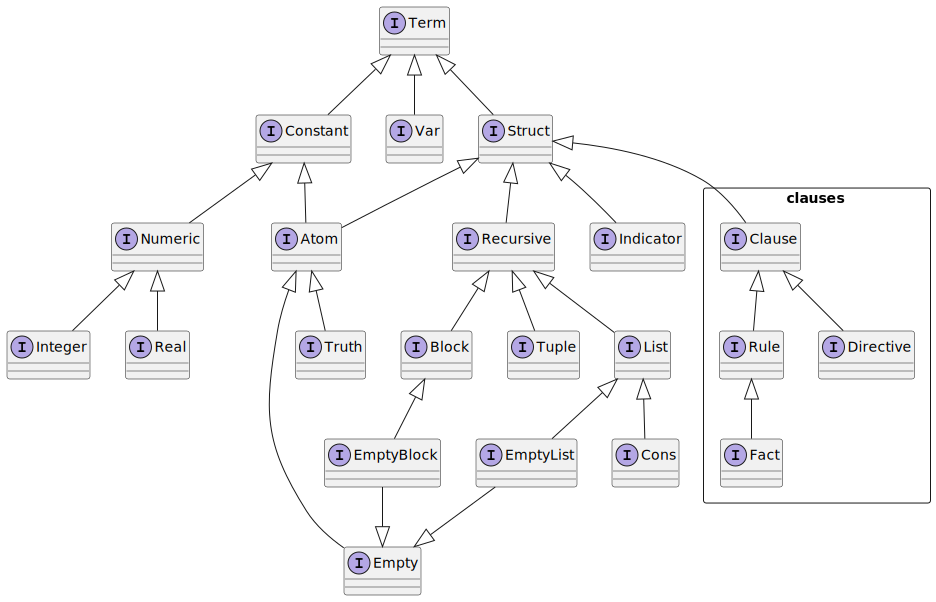
\includegraphics[width=.7\linewidth]{figures/term-hierarchy.pdf}
        \caption{Term's type hierarchy in \twopkt{}}
        \label{fig:term-hierarchy}
    \end{figure}

    \framebreak

    \begin{itemize}
        \item Set of interrelated interfaces for knowledge representation in \twopkt{}

        \bigskip

        \item \kt{Term} is the super-type of all terms and \alert{clauses} (Prolog trick)
        %
        \begin{description}
            \item[\kt{Var}] --- type for logic variables
            \item[\kt{Number}] --- type for numeric constants
            \item[\kt{Atom}] --- type for alphanumeric constants (strings)
            \item[\kt{Struct}] --- type for structures
            \item[\kt{List}] --- type for lists
            \item[\kt{Tuple}] --- type for conjunctions
            \item[\kt{Clause}] --- type for clauses
        \end{description}

        \framebreak

        \item All sub-types of \kt{Term}:
        %
        \begin{itemize}
            \item are strictly \alert{immutable} (i.e. one cannot alter a term/clause)
            \item come with a number of \alert{static factory} methods letting the user instantiate them
            %
            \begin{itemize}
                \item most commonly \kt{<Type>.\alert{of}(<args>)}
                \item they won't let you instantiate invalid terms or clauses :)
                \item they guarantee the term to be of the \alert{most adequate} sub-type
            \end{itemize}
        \end{itemize}

        \bigskip

        \item In the following exercises you will mostly need to create terms
        %
        \begin{itemize}
            \item use the map on figure \ref{fig:term-hierarchy} to know \alert{which} types exist
            \item have a look to \cite{Ciatto20212pktPresentation} for detailed API description
        \end{itemize}
    \end{itemize}
\end{frame}

\subsubsection{Exercises on terms}

\begin{frame}{About Exercises}

    \begin{block}{Repository}
        \centering
        \url{https://gitlab.com/pika-lab/courses/ise/ay2122/lab-1}
    \end{block}
    
\end{frame}

\startExercise{}

\begin{frame}{\currentExercise{} -- Terms construction}
    \label{slide:first-exercise-on-terms}

    \begin{block}{Goal}
        Understand the basics of terms construction in \twopkt{}
    \end{block}
    
\end{frame}

\startExercise{}

\begin{frame}{\currentExercise{} -- Herbrand Universe}
    \label{slide:second-exercise-on-terms}

    \begin{block}{Goal}
        \begin{itemize}
            \item Implement the algorithm for constructing the Herbrand Universe \ldots
            %
            \begin{itemize}
                \item \ldots spawned by a set of functors and their arities (provided as arguments)
            \end{itemize}

            \item Use the algorithm from slide \ref{slide:herbrand} as a reference
            
            \item Since $\mathcal{H}_\infty$ may be of infinite cardinality\ldots
            %
            \begin{itemize}
                \item \ldots you'll actually implement the algorithm for computing $\mathcal{H}_i$
                %
                \begin{itemize}
                    \item where $i$ is provided as argument
                \end{itemize}
            \end{itemize}
        \end{itemize}
    \end{block}
\end{frame}

\subsubsection{Exercises on Horn clauses}

\startExercise{}

\begin{frame}{\currentExercise{} -- Clauses construction}
    \label{slide:first-exercise-on-clauses}
    \begin{block}{Goal}
        Understand the basics of clauses and theories construction in \twopkt{}
    \end{block}
    
\end{frame}

\startExercise{}

\begin{frame}{\currentExercise{} -- Theory Analysis}
    \label{slide:second-exercise-on-clauses}
    \begin{block}{Goal}
        \begin{itemize}
            \item Write an algorithm aimed at inspecting a theory, in order to compute:
            %
            \begin{itemize}
                \item the set $\mathcal{P}$ of predicate names (predications)
                \item the set $\mathcal{F}$ of function names (functors)
                \item the set $\mathcal{X}$ of variables names 
            \end{itemize}
            \item It should work \alert{for any given theory}
        \end{itemize}
    \end{block}
\end{frame}

\subsubsection{Exercises on representations}

\startExercise{}

\begin{frame}{\currentExercise{} -- Relationalization}
    \begin{block}{Goal}
        \begin{itemize}
            \item Write an algorithm aimed at relationalising a theory in propositional form
            
            \item It should work \alert{for any given theory}
            
            \item The algorithm may accept as input:
            %
            \begin{itemize}
                \item a theory, assumed in propositional form
                \item the predication used to represent instances, in the propositional theory
                \item the names of the attributes (which may be implicit in the propositional theory)
            \end{itemize}
        \end{itemize}
    \end{block}
\end{frame}

%===============================================================================
\section{Inference}
%===============================================================================

%===============================================================================
\subsection{Premises}
%===============================================================================

\begin{frame}{Lecture Goals}
    \begin{itemize}
        \item Understand basic notions concerning the \alert{manipulation} of Horn clauses
        %
        \begin{itemize}
            \item substitutions
            \item unification and (most general) unifiers
        \end{itemize}

        \vfill

        \item Understand how these notions can be exploited for \alert{automated inference}
        %
        \begin{itemize}
            \item using the SL\ccite{Robinson1965} resolution principle\ldots
            \item \ldots as suggested by \cite{KowVan1970} (SLD)
        \end{itemize}

        \vfill

        \item Understand the notion of \alert{proof tree}
        %
        \begin{itemize}
            \item and the different possible strategies for its \alert{exploration}
        \end{itemize}
    \end{itemize}
\end{frame}

%===============================================================================
\subsection{Substitutions and their Application to Logic Formul\ae{}}
%===============================================================================

\begin{frame}{Overview}
    \begin{itemize}
        \item[$\checkmark$] Three main ingredients:
        %
        \begin{description}\small
            \item[terms] --- for representing entities
            \item[predicates] --- for representing statements about entities
            \item[clauses] --- for representing properties of entities or relations among them
        \end{description}

        \vfill

        \item[$\checkmark$] Many ways of representing knowledge through them:
        %
        \begin{description}\small
            \item[extensional vs. intensional] $\approx$ explicitly vs. implicitly
            \item[propositional vs. relational] $\approx$ in tabular form vs. as a graph
        \end{description}

        \vfill

        \item One powerful tool:
        %
        \begin{description}\small
            \item[resolution] --- allowing for \alert{intensional} representations, programming, reasoning, \ldots
        \end{description}

        \vfill

        \item[$\rightarrow$] Two fundamental mechanisms for manipulating knowledge:
        %
        \begin{description}\small
            \item[substitution application] $\approx$ rewriting a formula by assigning variables
            \item[most general unifier] $\approx$ computing the substitution making 2 formul\ae{} equal
        \end{description}
    \end{itemize}
\end{frame}

\subsubsection{Substitutions}

\begin{frame}[allowframebreaks]{Substitutions}
    \begin{block}{Purpose}\centering
        Denoting variables assignemnts
    \end{block}
    %
    \begin{block}{Informal definition}
        A (possibly \emph{empty}) set of \alert{variable--term} pairs
    \end{block}
    %
    \begin{alertblock}{Formal syntax\hfill\textbf{\footnotesize(same syntactic notation as in \cite{lectures:ise-kr})}}
        \begin{center}
            $\begin{array}{rcl}
                \meta{Substitution} & := & \terminal{\varnothing} \mid \terminal{\{} \meta{Assignemnts} \terminal{\}}
                \\
                \meta{Assignments} & := & \meta{Assignment} \mid \meta{Assignments} \terminal{,} \meta{Assignments}
                \\
                \meta{Assignment} & := & \meta{Variable} \terminal{\mapsto} \meta{Term}
                \\
                \meta{Term} & := & \text{see lecture \cite{lectures:ise-kr}}
                \\
                \meta{Variable} & := & \text{see lecture \cite{lectures:ise-kr}}
            \end{array}$
        \end{center}
    \end{alertblock}

    \begin{exampleblock}{Examples}
        \begin{description}
            \item[$\varnothing$] --- the empty substitution (no variable to be assigned)
            \item[$\{ \variable{X} \mapsto \functor{a} \}$] --- the substitution assigning variable $\variable{X}$ with the constant $\functor{a}$
            \item[$\{ \variable{X} \mapsto \functor{a}, \variable{Y} \mapsto \functor{b} \}$] --- the substitution assigning 
            %
            \begin{itemize}
                \item variable $\variable{X}$ with the constant $\functor{a}$, and
                \item variable $\variable{Y}$ with the constant $\functor{b}$ 
            \end{itemize} 
        \end{description}
    \end{exampleblock}
\end{frame}

\subsubsection{Substitution Application}

\begin{frame}[allowframebreaks]{Applying Substitutions to Logic Formul\ae{}}
    \begin{block}{Purpose}\centering
        Actually assigning some formula's variables with some values, as denoted by some given substitution
    \end{block}
    %
    \begin{block}{Informal definition}
        The operation by which 
        %
        \begin{enumerate}
            \item a formula (i.e. a term, a predicate, or a Horn cluase) \ldots
            \item \ldots is \alert{rewritten} \ldots
            \item \ldots by \alert{replacing} all variables therein contained \ldots
            \item \ldots with some other \alert{terms}, as prescribed by a given \alert{substitution}
        \end{enumerate}
    \end{block}
    %
    \begin{block}{Notation}
        \begin{itemize}
            \item We denote by 
            %
            \[ \Phi / \sigma \qquad \equiv \Phi'\]
            %
            the operation of applying a substitution $\sigma$ to some formula $\Phi$
            %
            \begin{itemize}
                \item hence producing a new formula $\Phi$
            \end{itemize}

            \item Notice that:
            %
            \begin{itemize}
                \item $(\cdot / \cdot)$ is a function mapping formul\ae{} and substitutions to other formul\ae{}
                \item we denote substitutions by lowercase greek letters such as $\sigma$, $\rho$, etc.
                \item we denote formul\ae{} by uppercase greek letters such as $\Phi$, $\Psi$, etc.
            \end{itemize} 
        \end{itemize}
    \end{block}
    %
    \begin{alertblock}{Formal definition}
        Let $\Phi, \Psi, \Psi', \Psi_1, \ldots, \Psi_n$ be logic formul\ae{} (i.e. terms, predicates, or a Horn cluases) of any sort, 
        %
        let $\predication{p}$ be a $n$-ary predication, let $\functor{f}$ be a $m$-ary functor, let $\functor{k}$ be a constant, let $t$ be a term of any sort,
        %
        and let $\sigma$ be a (possibly empty) substitution;
        %
        then
        
        $$\Phi / \sigma = \begin{cases}
            \Psi / \sigma \Leftarrow \Psi' / \sigma & \text{if} ~ \Phi \equiv \Psi \Leftarrow \Psi'
            \\
            \Psi / \sigma \wedge \Psi' / \sigma & \text{if} ~ \Phi \equiv \Psi \wedge \Psi'
            \\
            \predication{p}(\Psi_1 / \sigma, \ldots, \Psi_n / \sigma) & \text{if} ~ \Phi \equiv \predication{p}(\psi_1, \ldots, \psi_n)
            \\
            \functor{f}(\Psi_1 / \sigma, \ldots, \Psi_m / \sigma) & \text{if} ~ \Phi \equiv \functor{f}(\psi_1, \ldots, \psi_m)
            \\
            \functor{k} & \text{if} ~ \Phi \equiv \functor{k}
            \\
            t & \text{if} ~ \Phi \equiv \variable{X} ~ \text{and} ~ (\variable{X} \mapsto t) \in \sigma
            \\
            \variable{X} & \text{if} ~ \Phi \equiv \variable{X} ~ \text{and} ~ (\variable{X} \mapsto t) \not\in \sigma
        \end{cases}$$
    \end{alertblock}

    \begin{exampleblock}{Examples}
        \begin{itemize}
            \item[] \alert{$\functor{f}(\variable{X}) \ /\  \varnothing$} $\equiv$ $\functor{f}(\variable{X})$
            %
            \begin{itemize}
                \item applying empty substitutions to formul\ae{} has no effect
            \end{itemize} 

            \item[] \alert{$\functor{k} \ /\  \sigma$} $\equiv$ $\functor{k}$
            %
            \begin{itemize}
                \item applying substitutions to constants has no effect
            \end{itemize} 

            \item[] \alert{$\predication{p}(X, \functor{f}(Y)) \ /\  \{ X \mapsto \functor{a}, Y \mapsto \functor{b} \}$} $\equiv$ $\predication{p}(\functor{a}, \functor{f}(\functor{b}))$
            %
            \begin{itemize}
                \item applying substitutions to formul\ae{} replaces the variables therein contained\ldots
            \end{itemize} 

            \item[] \alert{$\predication{p}(X, \functor{f}(Y)) \ /\  \{ X \mapsto \functor{a} \}$} $\equiv$ $\predication{p}(\functor{a}, \functor{f}(Y))$
            %
            \begin{itemize}
                \item \ldots provided that the variable is contained in the substitution\ldots
            \end{itemize} 

            \item[] \alert{$\predication{p}(X, \functor{f}(Y)) \ /\  \{ X \mapsto \functor{a}, Z \mapsto \functor{b} \}$} $\equiv$ $\predication{p}(\functor{a}, \functor{f}(Y))$
            %
            \begin{itemize}
                \item \ldots and in the formula
            \end{itemize} 
        \end{itemize}
    \end{exampleblock}
\end{frame}

\subsubsection{Refreshing Formul\ae{}}

\begin{frame}[allowframebreaks]{Refreshing Formul\ae{}}
    \begin{block}{Purpose}
        Allowing a formula to be re-used in different contexts, avoiding undesired variable assignments 
        %
        \begin{itemize}
            \item this is not relevant in theory, but very important in practice
        \end{itemize}
    \end{block}
    %
    \begin{block}{Informal definition}
        A formula is \alert{refreshed} by 
        %
        \begin{itemize}
            \item \emph{consistently} replacing each variable therein contained
            \item with some \emph{bare new}\footnote{never used before} variable of similar name 
        \end{itemize}
    \end{block}
    %
    \begin{alertblock}{Formal definition}
        Let 
        %
        \begin{itemize}
            \item \alert{$\Phi$} be a formula (i.e. term, predicate, or Horn cluase) of any sort 
            \item \alert{$\rho = \{ \variable{X} \mapsto \hat{\variable{X}} \mid \forall \variable{X} \in \Phi \}$} be the refreshing substitution for $\Phi$
            %
            \begin{itemize}\small
                \item where $\hat{\variable{X}}$ is a variable which has \alert{never been used before}
            \end{itemize} 
        \end{itemize}
        %
        then we define ``refreshing $\Phi$'' as the operation of applying $\rho$ to $\Phi$:hat
        %
        \begin{center}
            $ \text{refresh}(\Phi) = \alert{\Phi / \rho} $
        \end{center}
    \end{alertblock}

    \begin{exampleblock}{Examples}
        \begin{multicols}{2}\small
            \begin{itemize}
                \item $\text{refresh}(\alert{\functor{f}(\variable{X}, \functor{g}(\variable{X}))})$ 
                \item $\text{refresh}(\alert{\predication{p}(\variable{X}, \functor{f}(\variable{Y}), \functor{g}(\variable{X}))})$ 
                \item $\text{refresh}(\alert{\predication{list}([\variable{H} \mid \variable{T} ])) \Leftarrow \predication{list}(\variable{T})})$ 
                
                \item[$=$] $\functor{f}(\hat{\variable{X}}, \functor{g}(\hat{\variable{X}}))$
                \item[$=$] $\predication{p}(\hat{\variable{X}}, \functor{f}(\hat{\variable{Y}}), \functor{g}(\hat{\variable{X}}))$
                \item[$=$] $\predication{list}([\hat{\variable{H}} \mid \hat{\variable{T} ]})) \Leftarrow \predication{list}(\hat{\variable{T}})$
            \end{itemize}
        \end{multicols}
    \end{exampleblock}
\end{frame}

\begin{frame}
    \begin{block}{Time to practice}
        \begin{itemize}
            \item You may start exercises about \alert{substitutions} now
            \item cf. slide \ref{slide:ex-sub}
        \end{itemize}
    \end{block}
\end{frame}

%===============================================================================
\subsection{Unification}
%===============================================================================

\begin{frame}{Overview}
    \begin{itemize}
        \item[$\checkmark$] Three main ingredients:
        %
        \begin{description}\small
            \item[terms] --- for representing entities
            \item[predicates] --- for representing statements about entities
            \item[clauses] --- for representing properties of entities or relations among them
        \end{description}

        \vfill

        \item[$\checkmark$] Many ways of representing knowledge through them:
        %
        \begin{description}\small
            \item[extensional vs. intensional] $\approx$ explicitly vs. implicitly
            \item[propositional vs. relational] $\approx$ in tabular form vs. as a graph
        \end{description}

        \vfill

        \item One powerful tool:
        %
        \begin{description}\small
            \item[resolution] --- allowing for \alert{intensional} representations, programming, reasoning, \ldots
        \end{description}

        \vfill

        \item[$\rightarrow$] Two fundamental mechanisms for manipulating knowledge:
        %
        \begin{description}\small
            \item[substitution application] $\approx$ rewriting a formula by assigning variables
            \item[most general unifier] $\approx$ computing the substitution making 2 formul\ae{} equal
        \end{description}
    \end{itemize}
\end{frame}

\begin{frame}[allowframebreaks]{Unification}
    \begin{block}{Purpose}
        Compute which variables assignment may let a given formula
        %
        \begin{itemize}
            \item be equal to another one
            \item hence fitting a particular context
        \end{itemize}
    \end{block}
    %
    \begin{block}{Informal definition}
        The operation by which one may compute
        %
        \begin{itemize}
            \item an \alert{unifier} among any two formul\ae{}
            %
            \begin{itemize}
                \item[ie] a \alert{substitution} making the two formul\ae{} \alert{syntactically equal}
            \end{itemize}

            \item or figure out that it is impossible to do so
        \end{itemize}
    \end{block}
    %
    \begin{alertblock}{Formal definition}
        \begin{center}
            $\text{unify}(\Phi, \Psi) = \begin{cases}
                \sigma & \text{if} ~ \exists \sigma : \Phi = \Psi / \sigma
                \\
                \Box & \text{otherwise}
            \end{cases}$
        \end{center}
        %
        where
        %
        \begin{itemize}
            \item \alert{$\sigma$} is called \alert{unifier} (i.e. the unifying substitution)
            \item \alert{$\Box$} denotes the \alert{failed} substitution (i.e. the impossibility to unify)
        \end{itemize}
    \end{alertblock}
\end{frame}

\subsubsection{Most General Unifier}

\begin{frame}{Most General Unifier (MGU)}

    \begin{alertblock}{Important remark}\centering
        In the general case, \alert{several} unifieriers may exist for any 2 formul\ae{}
    \end{alertblock}
    %
    \begin{exampleblock}{Try unifying $\predication{p}(\functor{a}, \variable{X}, \variable{X})$ and $\predication{p}(\variable{A}, \variable{B}, \variable{C})$}
        \begin{itemize}
            \item $\{ \variable{A} \mapsto \functor{a}, \variable{B} \mapsto \functor{a}, \variable{C} \mapsto \functor{a}, \variable{X} \mapsto \functor{a} \}$
            \item $\{ \variable{A} \mapsto \functor{a}, \variable{B} \mapsto \functor{b}, \variable{C} \mapsto \functor{b}, \variable{X} \mapsto \functor{b} \}$
            \item $\{ \variable{A} \mapsto \functor{a}, \variable{B} \mapsto \functor{c}, \variable{C} \mapsto \functor{c}, \variable{X} \mapsto \functor{c} \}$
            \item[$\vdots$]
            \item \alert{$\{ \variable{A} \mapsto \functor{a}, \variable{B} \mapsto \variable{X}, \variable{C} \mapsto \variable{X} \}$} \hint{this is more general}
        \end{itemize}
    \end{exampleblock} 
    %
    \begin{block}{Which unifier?}
        We're commonly interested in the \alert{most general} unifier!
    \end{block}
\end{frame}

\begin{frame}{When do Formul\ae{} Unify? A.k.a. how to compute MGU} 
    \begin{block}{Formal definition}
        \begin{adjustbox}{width=\textwidth} 
            \begin{tabular}{c||c|c|c}
                $\text{mgu}(\Phi,\Psi)$ & $\Phi \equiv \functor{c}$ & $\Phi \equiv \variable{X}$ & $\Phi \equiv f(t_1, \ldots, t_n)$
                \\
                \hline\hline
                $\Psi \equiv \functor{k}$ & $\begin{cases} \varnothing & \text{if} ~ \functor{c} = \functor{k} \\ \Box & \text{if} ~ \functor{c} \neq \functor{k} \end{cases} $ & $\{\variable{X} \mapsto \functor{k}\}$ & $\Box$
                \\
                \hline
                $\Psi \equiv \variable{Y}$ & $\{\variable{Y} \mapsto \functor{c}\}$ & $\{\variable{X} \mapsto \variable{Y}\}$ & $\{\variable{Y} \mapsto f(t_1, \ldots, t_n)\}$
                \\
                \hline
                $\Psi \equiv g(x_1, \ldots, x_m)$ & $\Box$ & $\{\variable{X} \mapsto g(x_1, \ldots, x_m)\}$ & $\begin{cases} \bigcup_i \text{mgu}(t_i, x_i) & \text{if} ~ f = g \wedge n = m \\ & \quad \wedge \not\exists j : \text{mgu}(t_j, x_j) = \Box \\ \Box & \text{otherwise} \end{cases}$
            \end{tabular}
        \end{adjustbox}
        %
        where
        %
        \begin{itemize}\small
            \item $\Phi, \Psi$ are arbitrary formul\ae{}
            \item $f, g$ are either functors or predications (or logic connectives of any sort)
            \item $t_1, \ldots, t_n$ and $x_1, \ldots, x_m$ are terms
        \end{itemize}
    \end{block}
    %
    \hint{commonly, we compute MGU via the algorithm proposed by \cite{MartelliM82}}
\end{frame}

\begin{frame}{Computing MGU -- Examples}
    \begin{itemize}
        \item $\text{mgu}(\quad 
            \alert{\functor{f}(\variable{X}, \functor{g}(2))} 
            \quad , \quad 
            \alert{\functor{f}(1, \functor{g}(\variable{Y}))}  
        \quad)$ 
        %
        \begin{itemize}
            \item[$=$] $\{ \variable{X} \mapsto 1, \variable{Y} \mapsto 2 \}$
        \end{itemize}

        \vfill

        \item $\text{mgu}(\quad 
            \alert{\predication{p}(\functor{a}, \functor{f}(\variable{X}), \variable{X})} 
            \quad , \quad 
            \alert{\predication{p}(\variable{A}, \variable{B}, \variable{A})} 
        \quad)$ 
        %
        \begin{itemize}
            \item[$=$] $\{ \variable{X} \mapsto \functor{a}, \variable{Y} \mapsto \functor{f}(\functor{a}), \variable{X} \mapsto \functor{a} \}$
        \end{itemize}

        \vfill

        \item $\text{mgu}(\enspace 
            \alert{\predication{sum}(\functor{s}(\functor{s}(\functor{s}(\functor{z}))), \functor{s}(\functor{z}), \functor{s}(\functor{s}(\functor{s}(\functor{s}(\functor{z})))))} 
            \enspace , \enspace 
            \alert{\predication{sum}(\functor{s}(\variable{N}), \variable{M}, \functor{s}(\variable{R}))} 
        \enspace)$ 
        %
        \begin{itemize}
            \item[$=$] $\{ \variable{N} \mapsto \functor{s}(\functor{s}(\functor{z})), \variable{M} \mapsto \functor{s}(\functor{z}), \variable{R} \mapsto \functor{s}(\functor{s}(\functor{s}(\functor{z}))) \}$
        \end{itemize}
    
    \end{itemize}
\end{frame}

\begin{frame}{Fun facts about Unification}
    \begin{itemize}
        \item Unification is far more general than logic programming alone
        
        \vfill

        \item Logic unification is one major contribution of LP to \alert{software engineering}\ccite{SterlingY96}
        
        \vfill

        \item Unification is what enables \alert{generics} and \alert{type inference} in strongly-typed languages
        %
        \kotlinimport{listings/unification-in-oop-langs.kt}
    \end{itemize}
\end{frame}

\begin{frame}
    \begin{block}{Time to practice}
        \begin{itemize}
            \item You may start exercises about \alert{unification} now
            \item cf. slide \ref{slide:ex-uni}
        \end{itemize}
    \end{block}
\end{frame}

%===============================================================================
\subsection{Satisfiability and Resolution}
%===============================================================================

\begin{frame}{Overview}
    \begin{itemize}
        \item[$\checkmark$] Three main ingredients:
        %
        \begin{description}\small
            \item[terms] --- for representing entities
            \item[predicates] --- for representing statements about entities
            \item[clauses] --- for representing properties of entities or relations among them
        \end{description}

        \vfill

        \item[$\checkmark$] Many ways of representing knowledge through them:
        %
        \begin{description}\small
            \item[extensional vs. intensional] $\approx$ explicitly vs. implicitly
            \item[propositional vs. relational] $\approx$ in tabular form vs. as a graph
        \end{description}

        \vfill

        \item[$\rightarrow$] One powerful tool:
        %
        \begin{description}\small
            \item[resolution] --- allowing for \alert{intensional} representations, programming, reasoning, \ldots
        \end{description}

        \vfill

        \item[$\checkmark$] Two fundamental mechanisms for manipulating knowledge:
        %
        \begin{description}\small
            \item[substitution application] $\approx$ rewriting a formula by assigning variables
            \item[most general unifier] $\approx$ computing the substitution making 2 formul\ae{} equal
        \end{description}
    \end{itemize}
\end{frame}

\begin{frame}{(Un-)Satisfiability}
    \begin{block}{Informal Definitions}
        A \alert{set} of logic formul\ae{} can be
        %
        \begin{description}
            \item[\textbf{un}satisfiable] --- meaning that a \alert{contradiction} may be derived from it
            %
            \begin{itemize}
                \item[eg] because it contains opposite statements
            \end{itemize} 

            \item[satisfiable] --- meaning that it is \emph{not} \textbf{un}satisfiable
            %
            \begin{itemize}
                \item[ie] no statement therein contained contradicts the others
            \end{itemize}  
        \end{description}
    \end{block}

    \begin{exampleblock}{Example of \textbf{un}satisfiable fomul\ae{}}
        \centering
        $\predication{triangle}(A, B, C) \Leftarrow (A \leq B + C) \wedge (B \leq A + C) \wedge (C \leq A + B)  \fullstop$
        \\
        $\predication{triangle}(10, 2, 3) \fullstop$
    \end{exampleblock}

\end{frame}

\begin{frame}[allowframebreaks]{Resolution = Deciding (Un-)Satisfiability}

    \begin{block}{Resolution Principles}
        \begin{itemize}
            \item Algorithms aimed at \alert{deciding} whether a given set of formul\ae{} is \textbf{un}satisfiable
            %
            \begin{itemize}
                \item by searching for a particular \alert{contradiction}
            \end{itemize}
        \end{itemize}
    \end{block}

    \begin{exampleblock}{SL resolution principle \cite{Robinson1965}}
        \begin{itemize}
            \item computes \textbf{un}satisfiability for any given set of FOL formul\ae{}
            %
            \begin{itemize}
                \item provided that they are in Skolemized form\footnote{cf. \uuurl{https://mathworld.wolfram.com/SkolemizedForm.html}}
            \end{itemize}
        \end{itemize}
    \end{exampleblock}

    \begin{exampleblock}{SL\textbf{D} resolution principle \cite{KowVan1970}}
        \begin{itemize}
            \item specialization for the SL resolution principle for Horn clauses
        \end{itemize}
    \end{exampleblock}

    \begin{alertblock}{How to prove a goal $\Phi$ against a theory $\mathcal{T}$?}
        \begin{itemize}
            \item Proof \alert{by contradiction} (a.k.a. \emph{reduction ab adsurdum})!
            %
            \begin{itemize}
                \item[ie] by proving that $\mathcal{T} \cup \{ \alert{\neg} \Phi \}$ is \alert{unsatisfiable}
            \end{itemize}
        \end{itemize}
    \end{alertblock}

    \begin{exampleblock}{General proof structure}
        \begin{enumerate}
            \item Assuming that $\mathcal{T}$ is satisfiable
            
            \item if we can prove $\mathcal{T} \cup \{ \alert{\neg} \Phi \}$ is unsatisfiable
            
            \item then we know that $\mathcal{T} \cup \{ \Phi \}$ is satisfiable
        \end{enumerate}
    \end{exampleblock}
\end{frame}

\subsubsection{SL Resolution}

\begin{frame}[allowframebreaks]{SL Resolution Principle\ccite{Robinson1965}}
    \begin{block}{\small Assumptions}
        \begin{itemize}\small
            \item Let $\mathcal{T} = \{ \Phi, \Psi, \ldots \}$ be a set of formul\ae{}
            %
            \begin{itemize}\footnotesize
                \item where each formula is a \alert{disjunction of literals} $\phi, \psi, \ldots$
                %
                \begin{itemize}\scriptsize
                    \item and where each literal may or may not be \alert{negated}
                \end{itemize}
            \end{itemize}
        \end{itemize}
    \end{block}
    %
    \begin{alertblock}{Resolution steps}
        \begin{enumerate}
            \item As long as there \alert{exist} any two formul\ae{} \alert{$\Phi$} and \alert{$\Psi$} such that
            %
            \begin{itemize}
                \item $\Phi \equiv \phi_1 \vee \ldots \vee \phi_{i-1} \vee \alert{\phi_i} \vee \phi_{i+1} \vee \ldots \vee \phi_{n}$
                \item $\Psi \equiv \psi_1 \vee \ldots \vee \psi_{j-1} \vee \alert{\neg\psi_j} \vee \psi_{j+1} \vee \ldots \vee \psi_{m}$
                \item $\exists \alert{\sigma} : \text{mgu}(\phi_i, \psi_j) = \alert{\sigma}$
            \end{itemize}

            \item Rewrite both $\Phi$ and $\Psi$ removing $\phi_i$ and $\psi_j$, respectively
            %
            \begin{itemize}
                \item $\Phi := (\phi_1 \vee \ldots \vee \alert{\phi_{i-1} \vee \phi_{i+1}} \vee \ldots \vee \phi_{n}) \alert{/ \sigma} $
                \item $\Psi := \psi_1 \vee \ldots \vee \alert{\psi_{j-1} \vee \psi_{j+1}} \vee \ldots \vee \psi_{m} \alert{/ \sigma}$
            \end{itemize}

            \item \alert{Stop} if either $\Phi$ or $\Psi$ are empty (i.e. if \alert{$n = 0 \vee m = 0$})
            %
            \begin{itemize}
                \item \alert{otherwise}, % apply \alert{$\sigma$} to \alert{all} formul\ae{} in $\mathcal{T}$, and 
                go to step 1
            \end{itemize}
            
        \end{enumerate}
    \end{alertblock}
    %
    \begin{alertblock}{The proof tree}
        \begin{itemize}
            \item SL resolution essentially explores a \alert{tree} of possible \alert{rewritings}
            \item At each step:
            %
            \begin{itemize}
                \item 2 rules are simplified
                \item some variables are assigned
            \end{itemize}
        \end{itemize}
    \end{alertblock}
\end{frame}

\begin{frame}{SL Resolution Principle -- Proof Tree Example}
    \begin{figure}
        \includegraphics[width=\linewidth]{figures/sl-path-all.pdf}
    \end{figure}
\end{frame}

\begin{frame}{SL Resolution Principle -- Search Space Size}
    \begin{itemize}
        \item The proof tree is potentially \alert{huge}
        %
        \begin{itemize}
            \item exploring it all in an \alert{uninformed} way is both costly, computationally
        \end{itemize}
        
        \vfill

        \item At each step, several couples of literals may be simplified
        %
        \begin{itemize}
            \item enumerating them all is computationally expensive as well
        \end{itemize}
        
        \vfill

        \item The ordering of rewritings is \alert{relevant}
        %
        \begin{itemize}
            \item simplifications are \alert{non-commutative}
        \end{itemize}

        \vfill

        \item FOL formul\ae{} are \alert{rarely} Skolemized and in \alert{disjunctive} form
        %
        \begin{itemize}
            \item conversely, Horn clauses are Skolemized \& disjunctive \alert{by definition}
        \end{itemize}
    \end{itemize}
\end{frame}

\subsubsection{SLD Resolution}

\begin{frame}{SLD Resolution Principle -- Overview}
    \begin{alertblock}{SL Resolution Principle for \textbf{Definite Clauses}}
        \begin{itemize}
            \item SLD just applied SL to Horn Clauses
            
            \item Horn clauses are Skolemized \& disjunctive \alert{by definition}
            
            \item Easier to select couples of literals to be simplified
            %
            \begin{itemize}
                \item any literal in the \alert{body} of any rule \alert{unifying} with the \alert{head} of any rule
            \end{itemize}

            \item[$\rightarrow$] Procedural interpretation of resolution\ccite{KowVan1970}
            %
            \begin{itemize}
                \item[ie] literals simplification $\approx$ function call
            \end{itemize}
        \end{itemize}
    \end{alertblock}
\end{frame}

\begin{frame}[allowframebreaks]{SLD Resolution Principle -- Example}
    \begin{block}{A theory (in implication form)}
        %
        \begin{multicols}{2}
            \begin{itemize}
                \item $\predication{parent}(\functor{abraham}, \functor{isaac}) \fullstop$
                \item $\predication{parent}(\functor{isaac}, \functor{jacob}) \fullstop$
                \item $\predication{parent}(\functor{sarah}, \functor{isaac}) \fullstop$
                \item $\predication{parent}(\functor{jacob}, \functor{joseph}) \fullstop$
                \item $\predication{parent}(\functor{jacob}, \functor{dan}) \fullstop$
                \item $\predication{parent}(\functor{jacob}, \functor{dinah}) \fullstop$
                \item $\predication{male}(\functor{abraham}) \fullstop$
                \item $\predication{male}(\functor{isaac}) \fullstop$
                \item $\predication{male}(\functor{jacob}) \fullstop$
                \item $\predication{male}(\functor{joseph}) \fullstop$
                \item $\predication{male}(\functor{dan}) \fullstop$
            \end{itemize}
        \end{multicols}
        %
        \begin{itemize}
            \item $\predication{son}(X, Y) \Leftarrow \predication{parent}(Y, X) \wedge \predication{male}(X) \fullstop$
            \item $\Leftarrow \predication{son}(S, \functor{jacob}) \fullstop$
        \end{itemize}
    \end{block}
\end{frame}

\begin{frame}[allowframebreaks]{SLD Resolution Principle -- Example}
    \begin{alertblock}{The same theory (in disjunctive form)}
        %
        \begin{multicols}{2}
            \begin{itemize}
                \item $\predication{parent}(\functor{abraham}, \functor{isaac}) \fullstop$
                \item $\predication{parent}(\functor{isaac}, \functor{jacob}) \fullstop$
                \item $\predication{parent}(\functor{sarah}, \functor{isaac}) \fullstop$
                \item $\predication{parent}(\functor{jacob}, \functor{joseph}) \fullstop$
                \item $\predication{parent}(\functor{jacob}, \functor{dan}) \fullstop$
                \item $\predication{parent}(\functor{jacob}, \functor{dinah}) \fullstop$
                \item $\predication{male}(\functor{abraham}) \fullstop$
                \item $\predication{male}(\functor{isaac}) \fullstop$
                \item $\predication{male}(\functor{jacob}) \fullstop$
                \item $\predication{male}(\functor{joseph}) \fullstop$
                \item $\predication{male}(\functor{dan}) \fullstop$
            \end{itemize}
        \end{multicols}
        %
        \begin{itemize}
            \item $\predication{son}(X, Y) \vee \neg\predication{parent}(Y, X) \vee \neg\predication{male}(X) \fullstop$
            \item $\neg\predication{son}(S, \functor{jacob}) \fullstop$
        \end{itemize}
    \end{alertblock}

    \begin{figure}
        \includegraphics[width=\linewidth]{figures/proof-tree.png}
        %
        \caption{Proof tree exploration subtended by the query $\Leftarrow \predication{son}(S, \functor{jacob}) \fullstop$}
    \end{figure}
\end{frame}

\begin{frame}[allowframebreaks]{About the Proof Tree Exploration}
    \begin{itemize}
        \item SL(D) is a \alert{non-deterministic} algorithm
        %
        \begin{itemize}
            \item[ie] at any given step, several choices may be taken 
            %
            \begin{itemize}
                \item[aka] different paths may be explored
            \end{itemize} 
        \end{itemize}

        \bigskip

        \item No prescription concerning which literals should be simplified first  
        %
        \begin{itemize}
            \item[aka] which rule to try first when multiple ones could apply?
        \end{itemize}

        \bigskip

        \item Possible ways to explore the proof tree:
        %
        \begin{description}
            \item[backward chaining] (a.k.a. \emph{goal-directed}) --- start from a goal and try to solve any sub-goal implying it, recursively
            \item[forward chaining] --- start from theory and try to infer anything that can be inferred from it
        \end{description}

        \framebreak

        \item Possible search strategies to explore the proof tree:
        %
        \begin{description}
            \item[depth first] --- explore most recent goals \alert{first}
            \item[breadth first] --- explore most recent goals \alert{last} 
            \item[$\vdots$] 
        \end{description}

        \bigskip

        \item Relevant \emph{properties} a given search strategy should have: 
        %
        \begin{description}
            \item[soundness] --- \alert{any} solution found by the strategy is \alert{correct}
            \item[completeness] --- the strategy enumerates \alert{all} correct solution
        \end{description}
    \end{itemize}
\end{frame}

\begin{frame}{Proof Tree Exploration -- Example}
    \begin{figure}
        \centering
        \includegraphics[width=.8\linewidth]{figures/exploration.pdf}
    \end{figure}
\end{frame}

\begin{frame}{Proof Tree Exploration -- Example (depth-first)}
    \begin{figure}
        \centering
        \includegraphics[width=.7\linewidth]{figures/exploration-df.pdf}
    \end{figure}
\end{frame}

\begin{frame}{Proof Tree Exploration -- Example (breadth-first)}
    \begin{figure}
        \centering
        \includegraphics[width=.7\linewidth]{figures/exploration-bf.pdf}
    \end{figure}
\end{frame}

% \subsubsubsection{Prolog}

\begin{frame}{Prolog's Proof Tree Exploration Strategy}
    \begin{itemize}
        \item Goal-directed, depth-first, sequential exploration strategy
        %
        \begin{itemize}
            \item may get stuck in recursive definitions
        \end{itemize}

        \vfill

        \item Goal-directed $\rightarrow$ \alert{procedural} interpretation of Prolog
        
        \vfill

        \item Depth-first $\approx$ \alert{left-most} goal first, \alert{top-most} rule first
        
        \vfill

        \item \alert{Backtracking} $\rightarrow$ sequential exploration
        %
        \begin{itemize}
            \item \emph{concurrent} implementations may get rid of backtracking
        \end{itemize}

        \vfill

        \item Support for \alert{side-effects} \emph{during} resolution
        %
        \begin{itemize}
            \item[eg] edits to the knowledge base (a.k.a. assertions and retractions)
            \item[eg] manipulation of exploration procedure (e.g. cut)
            \item[eg] I/O facilities via streams (a.k.a. sources and sinks) 
        \end{itemize}
    \end{itemize}
\end{frame}

%===============================================================================
\subsection{Exercises}
%===============================================================================

\begin{frame}[allowframebreaks]{All exercises}

    \begin{alertblock}{Repository}
        \centering
        \url{https://gitlab.com/pika-lab/courses/ise/ay2122/lab-2}
    \end{alertblock}

    \begin{block}{Exercises about \textbf{substitutions}}
        \label{slide:ex-sub}
        \begin{description}
            \startExercise
            \item[\currentExercise] is about substitutions and their application 
            \startExercise
            \item[\currentExercise] is about clauses and their refreshing
            \startExercise
            \item[\currentExercise] is about substitutions and their merging
        \end{description}
    \end{block}
    %
    \begin{block}{Exercises about \textbf{unification}}
        \label{slide:ex-uni}
        \begin{description}
            \startExercise
            \item[\currentExercise] is about MGU and its computation
            \startExercise
            \item[\currentExercise] is about theories and their exploitation for clause retrieval via unification
        \end{description}
    \end{block}
    %
    \begin{block}{Exercises about \textbf{resolution}}
        \label{slide:ex-res}
        \begin{description}
            \startExercise
            \item[\currentExercise] is about depth-first resolution strategies
            %
            \begin{itemize}
                \item here you should implement a depth-first, Prolog-like solver (supporting no side-effects)
            \end{itemize} 

            \startExercise
            \item[\currentExercise] is about smarter resolution strategies
            %
            \begin{itemize}
                \item here you should implement a Prolog-like solver (supporting no side-effects) \ldots
                \item \ldots which avoids getting stuck in simple recursive definitions such as:
                %
                \begin{center}
                    $\begin{array}{l}
                        \predication{nat}(\functor{s}(X)) \Leftarrow \predication{nat}(X) \fullstop
                        \\
                        \predication{nat}(\functor{z}) \fullstop
                    \end{array}$
                \end{center}
            \end{itemize} 
        \end{description}
    \end{block}
\end{frame}

%===============================================================================
\section*{}
%===============================================================================

%/////////
\frame{\titlepage}
%/////////

%===============================================================================
\section*{\refname}
%===============================================================================

%%%%
\setbeamertemplate{page number in head/foot}{}
%/////////
\begin{frame}[t,allowframebreaks,noframenumbering]{\refname}
%	\tiny
    \scriptsize
%	\footnotesize
    \bibliographystyle{apalike-AMS}
    \bibliography{eass23-cl-in-mas}
\end{frame}
%/////////

%%%%%%%%%%%%%%%%%%%%%%%%%%%%%%%%%%%%%%%%%%%%%%%%%%%%%%%%%%%%%%%%%%%%%%%%%%%%%%%%
\end{document}
%%%%%%%%%%%%%%%%%%%%%%%%%%%%%%%%%%%%%%%%%%%%%%%%%%%%%%%%%%%%%%%%%%%%%%%%%%%%%%%%
